\section{Iterative Refinement of the Unsat Core}
Similar to all other core extractors, our algorithm cannot generate a
minimal core in one execution. To obtain a smaller core, we need to
re-execute our tool with the core obtained in the current
iteration. We describe two heuristics that are applied to our
algorithm to increase the probability to generate a smaller core in
the next iteration. 

After eliminating all redundant polynomials, we can call our GB engine
with the new core. A effective heuristic should enhance the
probability that the refutation "1" is composed by fewer polynomials. 
In our GB computing algorithm, we use a strategy to pick critical
pairs such that polynomials with  larger indexes get involved as late
as possible: 
$$(f_1,f_2)\to(f_1,f_3)\to(f_2,f_3)\to(f_1,f_4)\to(f_2,f_4)\to\cdots$$

Meanwhile, for the reduction process $Spoly(f_i,f_j)\xrightarrow{F}_+
f_{new}$, we pick divisor polynomials from $F$ following the order of
polynomial indexes. Therefore, by renaming the polynomial indexes, we
can increase the likelihood they are selected into the unsat core. 
We use 2 criteria to increase the probability that a polynomial is
included in the refutation tree.  One corresponds to the \emph{refutation distance},
whereas the other corresponds to the frequency that
a polynomial appears in refutation tree. 

\begin{definition}
\emph{Refutation distance} in a refutation tree corresponds to the number of arcs on
the shortest path from refutation "1" to a leaf
polynomial.
\end{definition}

Polynomials with shorter refutation distance are used as
divisors in later stages of polynomial reductions, which indicates
they will generally have lower degree leading terms.  
This is because we are assuming a degree-lexicographic order, and
successive term cancellations reduce the degree of the remainders. So
polynomials with lower degree leading terms are more  likely to be
used for reduction, such that the probability that they appear in
the refutation tree is larger.  

Similarly, the motivation for \emph{frequency of appearance} of $f_i$ in
the refutation tree is as follows: polynomials appearing frequently in
the refutation tree also indicates that they have some properties
(leading terms) that make them "favourable" in the unsat core
selection. For example, their leading terms may contain variables
that are require them to be included in the minimal core. 

We apply both heuristics: we sort the polynomials in the core
by the refutation distance criterion, and use the frequency criterion as
the tiebreaker. The following example illustrates our heuristic. 


%\vspace{5mm}\\
\begin{example} 
Consider a set of 6 polynomials over $\F_2$ of an
infeasible instance.
\begin{align*}
f_1 &: x_1x_3+x_3\\
f_2 &: x_2 + 1\\
f_3 &: x_2x_3+x_2\\
f_4 &: x_2x_3\\
f_5 &: x_2x_3 + x_2 + x_3 + 1\\
f_6 &: x_1x_2x_3 +x_1x_3
\end{align*}

After the first iteration, we get a tree of refutation as shown in Fig.\ref{fig:refine}(a). 
\begin{figure}[hbt]
\centering
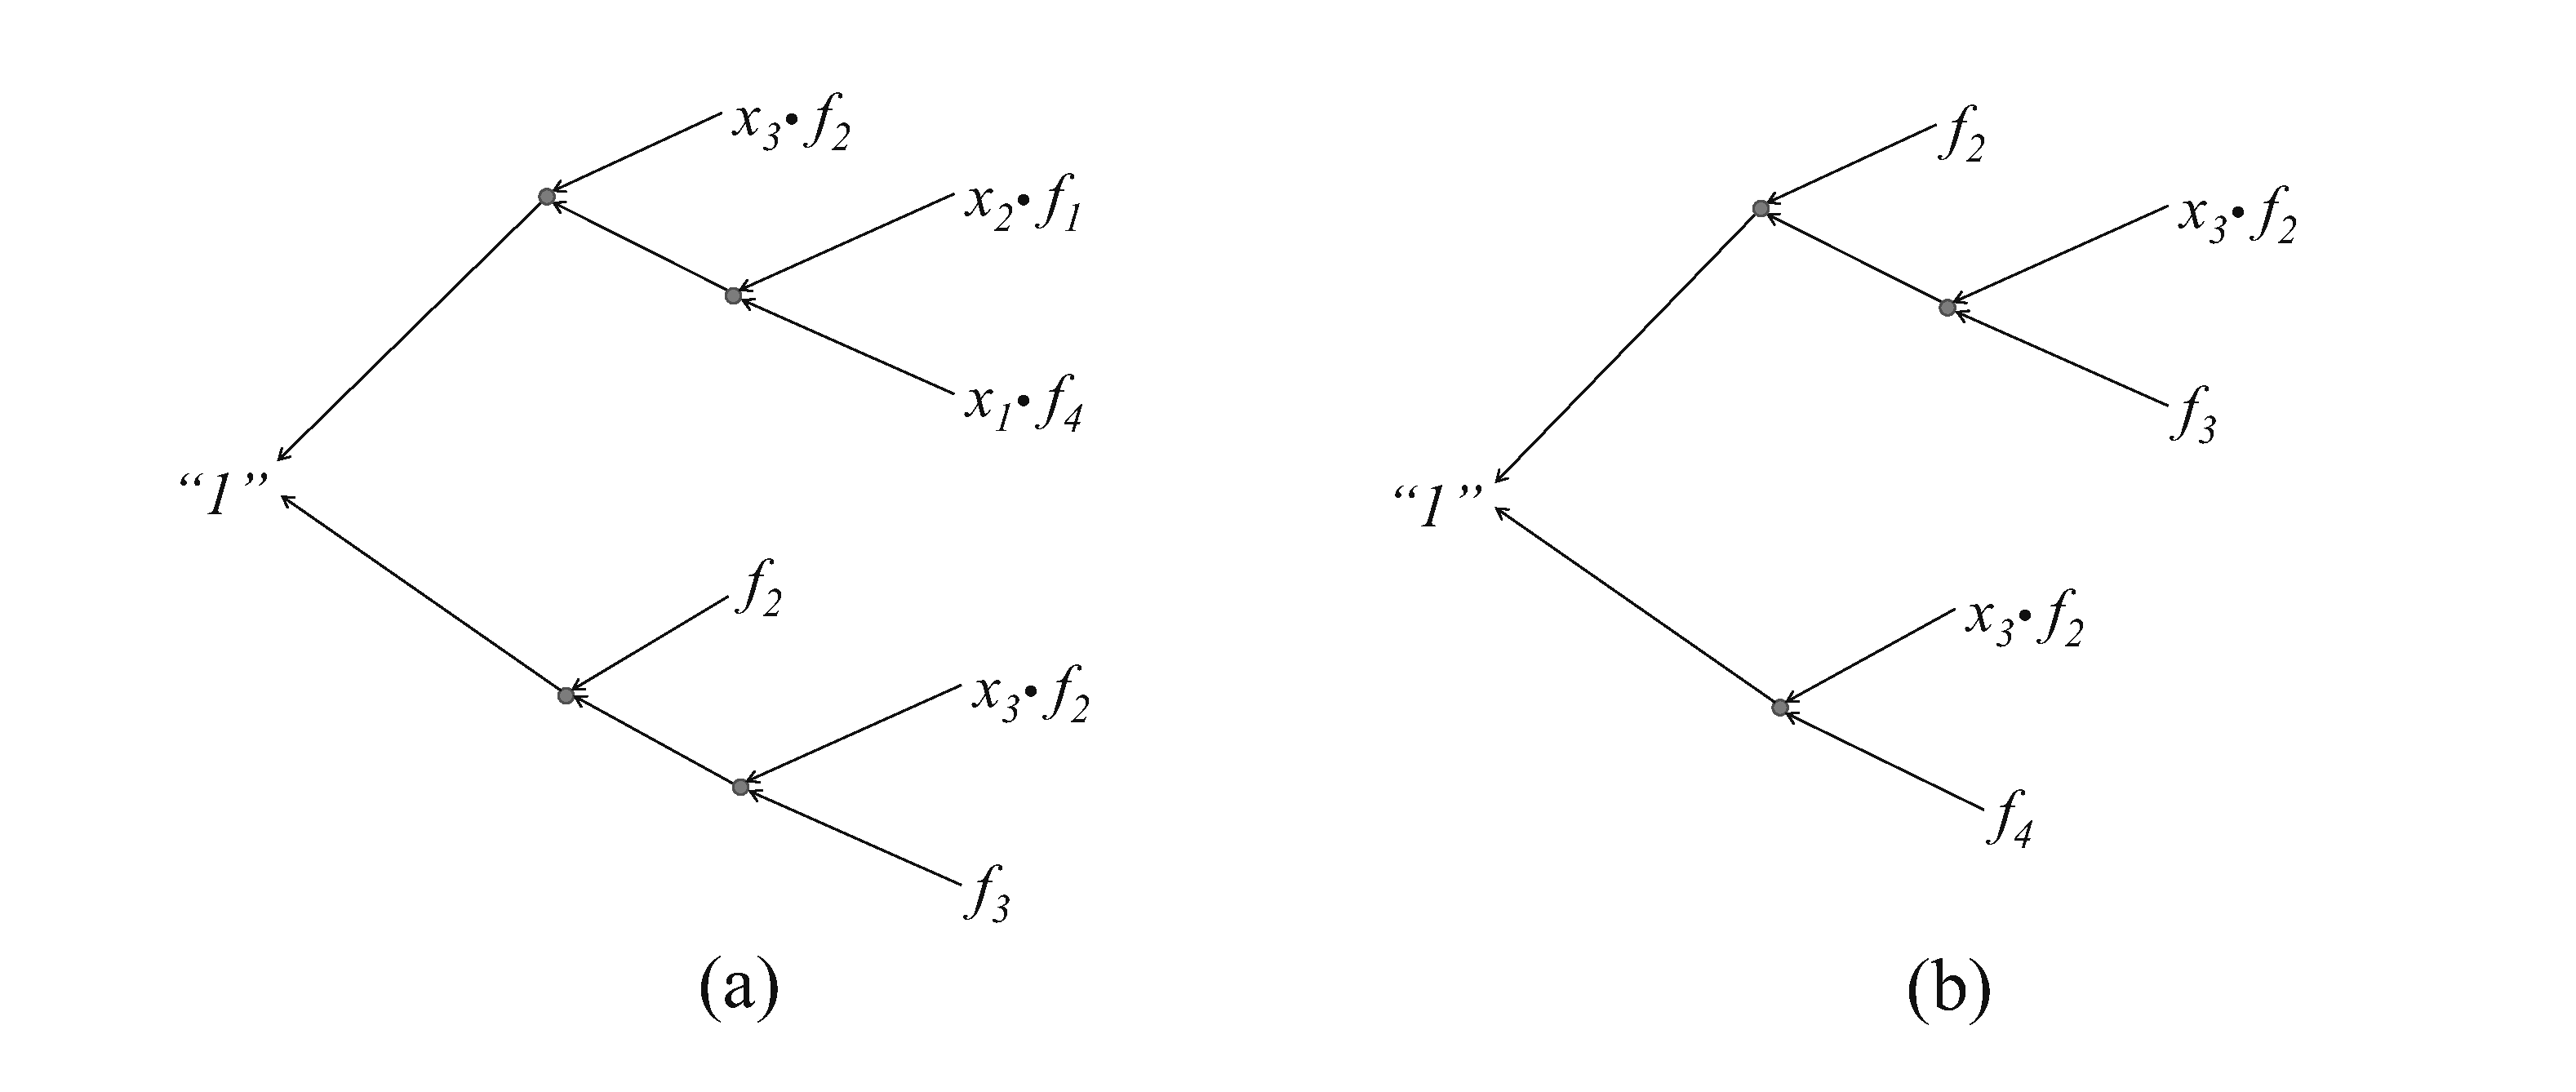
\includegraphics[scale=0.25]{SAT2016_xiaojun/core_refine.eps}
\caption{Refutation trees of core refinement example}
\label{fig:refine}
\end{figure}

The shortest "Distance" corresponds to that of $f_2$ to "1", which is
2 levels. So, we reorder $f_2$ to be the polynomial with the shortest
index. The "distance" and "frequency" for other polynomials are
identical, so we keep their ordering untouched. We re-index the
polynomial set 
$$f_1'=f_2, f_2' = f_1, f_3' = f_3, f_4' = f_4$$
and apply our GB-core algorithm on $\{f_1',f_2',f_3',f_4'\}$. The
result is shown in Fig.\ref{fig:refine}(b). We reach a fixpoint, and
the core $\{f_1', f_3', f_4'\} = \{f_2,f_3,f_4\}$ is proved to be
minimal. 
\end{example}
